\newpage
\section{Metodologia Experimental}

    \subsection{Materiais}
        O material utilizado para realização do experimento foi:

        \begin{itemize}
            \item U-2970A Gerador de dados;
            \item U-2970B Formato de dados;
            \item U-2970C Modulador balanceado duplo;
            \item U-2970D Deslocamento de fase da portadora;
            \item U-2970E Oscilador Controlado por Tensão;
            \item U-2970F Regenerador de clock de dados;
            \item U-2970G Recuperador de dados;
            \item U-2970H Receptor de dados;
            \item U-2970L Circuito de sintonia;
            \item U-2970M Fonte de alimentação;
            \item 1 Osciloscópio de 2 canais.
        \end{itemize}

        Para execução do experimento, faz-se necessário executar os passos abaixo, de acordo com o roteiro disponibilizado em sala de aula.

    \subsection{Métodos}
        \subsubsection{Método 1: Transmissão de pelo menos duas formas de onda de dados com a metade da taxa}
                      
            \begin{enumerate}
                \item Conectar o equipamento como mostrado na figura \ref{fig:montagem}-a.
                
                \item As formas de onda A e B do módulo formatação dos dados U-2970B são as duas formas de ondas com metade da taxa. A forma de onda A transmite os primeiros (MSB), terceiros, quintos e sétimos bits dos dados originais; a forma de onda de B transmite os outros.
                
                \item Configurar os osciloscópio com trigger externo da palavra de clock para mostrar um ciclo daquele clock. Então transferir o CH1 para a saída NRZ do módulo formato de dados e o CH2 primeiro para a saída A e depois para a saída B para verificar que as saídas A e B comportam-se como descrito acima.
                
                \item Depois procure pela saída do integrador no módulo de recuperação dos dados U-2970G. Configurar a palavra de dados tendo 0’s e 1’s transmitidos por cada um dos canais A e B tal
                como 00110011. Ajustar o controle de polarização do integrador para equalizar o negativo e o positivo de cada forma de onda.
                
                \item Deve agora ser possível enviar dados do módulo fonte para o módulo de recepção. A operação do clock da palavra recuperada pode ser checado pela interrupção da conecção do bit de clock
                e observando que o deslocamento da palavra de saída é corrigida quando o reconhecimento da palavra é recebido. (Observar que o reconhecimento sempre é sinalizado pela lâmpada A desde que ainda não tenhamos introduzido uma portadora de referência).
            \end{enumerate}
    
                 \begin{figure}[H]
                   \centering
                   \caption{a) Princípio do QPSK (dois sinais de meia taxa). b) Transmissor QPSK, controle de dois sinais de dados com moduladores separados cujas saídas produzem o sinal QPSK.}
                   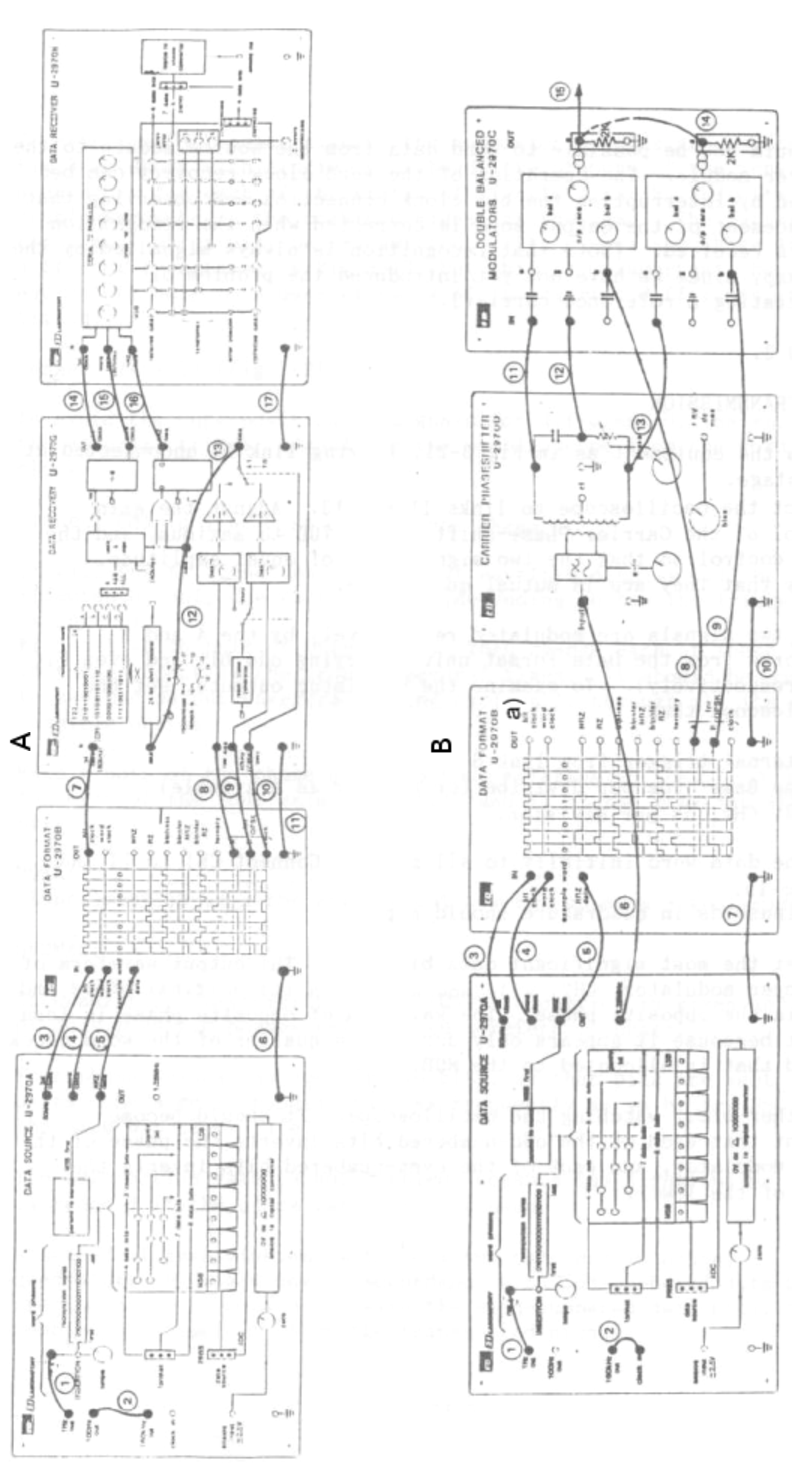
\includegraphics[scale=0.9]{montagem}
                   
                   \small Fonte: Jacob, J. L., Roteiro de laboratório 18; Universidade Estadual de Londrina, 2016.
                   \label{fig:montagem}
                  \end{figure}
                  
        \subsubsection{Método 2: Transmissão QSPK}

                    
            \begin{enumerate}
                \item Configurar o equipamento como na figura \ref{fig:montagem}-b, deixando a ligação 14 desconectada neste estágio. 
                
                \item Conectar o osciloscópio nas ligações 11 e 13. Ajustar o controle de ganho do deslocamento de fase da portadora U-2970D no máximo e o controle de fase tal que os dois sinais tornem-se
                de amplitudes iguais. Verificar que eles são em quadratura mútua.
                
                \item Estes dois sinais são modulados respectivamente pelas formas de onda A e B da unidade de formatação de dados (carregando dados de bits impares e de bits pares respectivamente). Para examinar a saída do modulador configurar o osciloscópio da seguinte forma:
                
                \begin{enumerate}
                  \item Trigger externo na ligação 6.
                  
                  \item Base de tempo: $1\mu s$ por divisão.
                  
                  \item CH1 e CH2: 5V/divisão.
                \end{enumerate}

                \item Configurar as palavras de dados inicialmente como tudo zero. Conectar CH1 na ligação 14 e CH2 na ligação 15.
                
                \item Duas senóides em quadratura devem aparecer.
                
                \item Agora configurar o bit de dados mais significativo para 1. A forma de onda de saída do modulador superior, CH2 aparecerá agora nesta fase original e também na fase oposta. A
                forma de onda da fase oposta é menos brilhante porque somente durante um quarto do período da palavra clock que é alocado no MSB.
                
                \item Configurar os outros bits observando o osciloscópio. Isto deve tornar evidente que cada combinação de bits impar inverte a fase do modulador superior e cada combinação de bits par inverte a fase do modulador inferior.
                
                \item Para fazer o sinal de quatro fases as saídas do modulador são combinadas. A figura \ref{fig:montagem}-b mostra com uma seta a saída do modulador separado para cada um dos estados dos sinais A e B e com duas setas os sinais combinados na carga. O último é o sinal que será transmitido. (Suas fases são mostradas com diferença de 45° daquelas na figura \ref{fig:montagem}-a, mas isto não é importante sendo equivalente somente a um quarto de ciclo de diferença da portadora em tempo).
                
                \item Conectar a ligação 14 (figura \ref{fig:montagem}-b).
                
                \item Para evitar a sobreposição de sinais para os diferentes pares de bits usa-se o sinal do trigger externo da palavra de clock para o osciloscópio.
                
                \item Conectar CH1 na ligação 6 como uma referência de fase.
                
                \item Agora será visto que a forma de onda de saída mostrada irá afetar somente um par de bits (dependendo de como o trigger é configurado).
                
                \item Descobrir qual é o par de bits. Em seguida trocar cada um desses bits por vez, repetindo o processo por várias vezes. Deve ser possível ver a forma de onda de saída que passa ciclicamente através de todas as suas quatro fases possíveis.
                
                \item Anotar as fases de saída relativa a referência CH1 para cada uma dos quatro valores 00, 01, 10 e 11 dos pares de bits relevantes.

            \end{enumerate}